\documentclass[a4paper,10pt,twocolumn]{article}

\usepackage[UTF8,fontset=fandol]{ctex}
\usepackage{amsmath,amssymb}
\usepackage{graphicx}
\usepackage{booktabs}
\usepackage{geometry}
\usepackage{hyperref}
\usepackage{caption}
\usepackage{array}
\usepackage{float}
\usepackage{xcolor}

\graphicspath{{./}{work4/}}

\geometry{a4paper,margin=1.7cm,columnsep=0.75cm}
\setlength{\parindent}{2em}
\setlength{\parskip}{0.25em}
\renewcommand{\arraystretch}{1.15}

\title{课程报告四：基于神经网络的《九章算术》语言模型与文本嵌入}
\author{方俊睿\\学号：3230104069}
\date{}

\begin{document}
\maketitle

\noindent 仓库地址：\url{https://github.com/Tomabsolute/Neul.git}

\section{实验背景介绍}
本实验面向《九章算术》文本训练小型神经网络语言模型，目标不是构建通用大语言模型，而是在课程规模内观察模型是否能够从古代数学文本中学习到稳定的题目、答案和数学词汇模式。附件文本包含题目与「答曰」后的解答。程序预处理时将原文中的异体写法统一为「答曰」，再抽取题面--答案对用于生成模型训练与评估。

实验包含两部分：第一部分为序列生成模型，采用字符级 LSTM 语言模型，在给定题面和「答曰：」提示后生成答案文本；第二部分为文本嵌入模型，采用 Skip-gram Negative Sampling 训练轻量 word2vec 式嵌入，通过近邻词观察模型是否捕捉到《九章算术》中的数学概念关系。

\section{实验任务与目标}
本实验的具体目标如下：
\begin{itemize}
  \item 从原始《九章算经》文本中自动识别题目与答案；
  \item 训练一个字符级 LSTM 序列生成模型，生成「答曰」后的答案；
  \item 训练一个文本嵌入模型，展示数学词汇或字符的相似关系；
  \item 记录训练损失、困惑度、答案关键词命中率与生成样例；
  \item 提供可在服务器上直接运行的脚本与报告。
\end{itemize}

\section{数据集与预处理}
\subsection{文本读取}
原始文件为 \texttt{work4/九章算经.txt}。该文件编码方式为 GB 2312，因此读取函数会依次尝试 \texttt{utf-8}、\texttt{gb2312}、\texttt{gb18030} 与 \texttt{gbk}。文本读取后进行以下标准化：
\begin{itemize}
  \item 将 Windows 换行统一为 \texttt{\textbackslash n}；
  \item 将原文中的异体写法统一为「答曰」；
  \item 合并多余空格和连续空行；
  \item 训练时按字符切分，去掉空白符。
\end{itemize}

\subsection{题答对抽取}
《九章算术》题目通常以「〔一〕」「〔二〕」等编号开头，答案由「答曰：」引出。脚本使用正则表达式切分编号块，并在每个块中查找「答曰：」。若找到答案，则构造
\[
\text{输入提示}=\text{题面}+\text{``答曰：''},\quad
\text{目标输出}=\text{答案文本}.
\]
抽取结果按随机种子划分为训练集和验证集，其中验证集比例为 15\%。这种划分能够检验模型对未见题目的续写能力。

\section{序列生成模型}
\subsection{模型结构}
序列生成部分采用字符级 LSTM。选择字符级建模的原因是《九章算术》包含大量古汉语数字、单位和术语，直接按字建模可以避免分词工具对繁体古文不稳定的问题。模型结构如下：

\begin{table}[H]
\centering
\small
\caption{字符级 LSTM 语言模型结构}
\begin{tabular}{c|c}
\toprule
模块 & 默认配置 \\
\midrule
输入 & 字符 ID 序列 \\
Embedding & 128 维 \\
LSTM & 2 层，隐藏维度 256 \\
Dropout & 0.2 \\
Linear & 隐藏状态映射到词表大小 \\
\bottomrule
\end{tabular}
\end{table}

模型在每个时间步预测下一个字符，损失函数为交叉熵：
\[
\mathcal{L}=-\sum_t \log p(x_{t+1}|x_{\le t}).
\]
推理时输入完整题面和「答曰：」，模型逐字符采样生成答案。采样温度默认为 0.75，以兼顾确定性和可读性。

\subsection{训练配置}
\begin{table}[H]
\centering
\small
\caption{LSTM 默认训练配置}
\begin{tabular}{c|c}
\toprule
项目 & 配置 \\
\midrule
训练文本 & 抽取出的题面--答案对 \\
序列长度 & 96 \\
Batch size & 128 \\
Epoch & 40，可在服务器上调大 \\
优化器 & AdamW \\
学习率 & $2\times10^{-3}$ \\
梯度裁剪 & 1.0 \\
设备 & CUDA / MPS / CPU 自动选择 \\
\bottomrule
\end{tabular}
\end{table}

\subsection{评价方式}
语言模型的数值指标包括验证集交叉熵和困惑度。为了更直接观察模型是否学到知识，脚本还在验证题目上生成答案，并计算答案关键词命中率。关键词主要来自数字和单位，例如「一、二、三、十、百、分、步、畝、頃、尺、升、斗」等。若生成文本覆盖至少一半答案关键词，则记为一次命中。

\section{文本嵌入模型}
\subsection{模型结构}
文本嵌入部分实现 Skip-gram Negative Sampling。给定中心字符 $w_t$，模型预测窗口内上下文字符 $w_c$，并用负采样近似 softmax。损失为：
\[
\mathcal{L}= -\log \sigma(v_{w_t}^{\top}u_{w_c})
-\sum_{i=1}^{K}\log \sigma(-v_{w_t}^{\top}u_{n_i}).
\]
其中 $K$ 为负样本数，默认取 8。训练完成后使用输入嵌入向量，并通过余弦相似度检索近邻。

\subsection{训练配置}
\begin{table}[H]
\centering
\small
\caption{Skip-gram 默认训练配置}
\begin{tabular}{c|c}
\toprule
项目 & 配置 \\
\midrule
Token 粒度 & 字符 \\
Embedding 维度 & 128 \\
窗口大小 & 4 \\
负样本数 & 8 \\
Batch size & 2048 \\
Epoch & 25，可在服务器上调大 \\
优化器 & AdamW \\
\bottomrule
\end{tabular}
\end{table}

\section{代码与运行方式}
实验代码位于 \texttt{work4/}：
\begin{itemize}
  \item \texttt{train\_lm.py}：训练 LSTM 语言模型；
  \item \texttt{generate\_answer.py}：加载模型并生成答案；
  \item \texttt{train\_word2vec.py}：训练 Skip-gram 文本嵌入；
  \item \texttt{run\_all\_experiments.sh}：一键运行两个实验；
  \item \texttt{src/}：数据处理、模型和画图工具。
\end{itemize}

一键运行命令为：
\begin{verbatim}
bash work4/run_all_experiments.sh
\end{verbatim}
服务器上可以使用：
\begin{verbatim}
LM_EPOCHS=80 EMB_EPOCHS=40 BATCH_SIZE=256 \
  bash work4/run_all_experiments.sh
\end{verbatim}

\section{实验结果展示}
训练完成后，LSTM 语言模型会输出 \texttt{metrics.json}、\texttt{history.csv}、\texttt{generation\_samples.md} 和训练曲线。嵌入模型会输出 \texttt{neighbors.md}、\texttt{neighbors.json} 与近邻可视化图。

\begin{table}[H]
\centering
\small
\caption{服务器训练结果记录表}
\begin{tabular}{c|c}
\toprule
项目 & 数值 \\
\midrule
题答对数量 & 见 \texttt{metrics.json} \\
验证集最优 loss & 见 \texttt{metrics.json} \\
验证集最优 PPL & 见 \texttt{metrics.json} \\
答案关键词命中率 & 见 \texttt{metrics.json} \\
LSTM 参数规模 & 约 1--2M，随词表略变 \\
\bottomrule
\end{tabular}
\end{table}

\begin{figure}[H]
\centering
\IfFileExists{results/lstm_lm/curves.png}
{
\includegraphics[width=\columnwidth]{results/lstm_lm/curves.png}}
{\fbox{\parbox{0.9\columnwidth}{\centering 服务器运行后生成 \texttt{results/lstm\_lm/curves.png}}}}
\caption{字符级 LSTM 训练曲线}
\end{figure}

\begin{figure}[H]
\centering
\IfFileExists{results/word2vec/neighbors.png}
{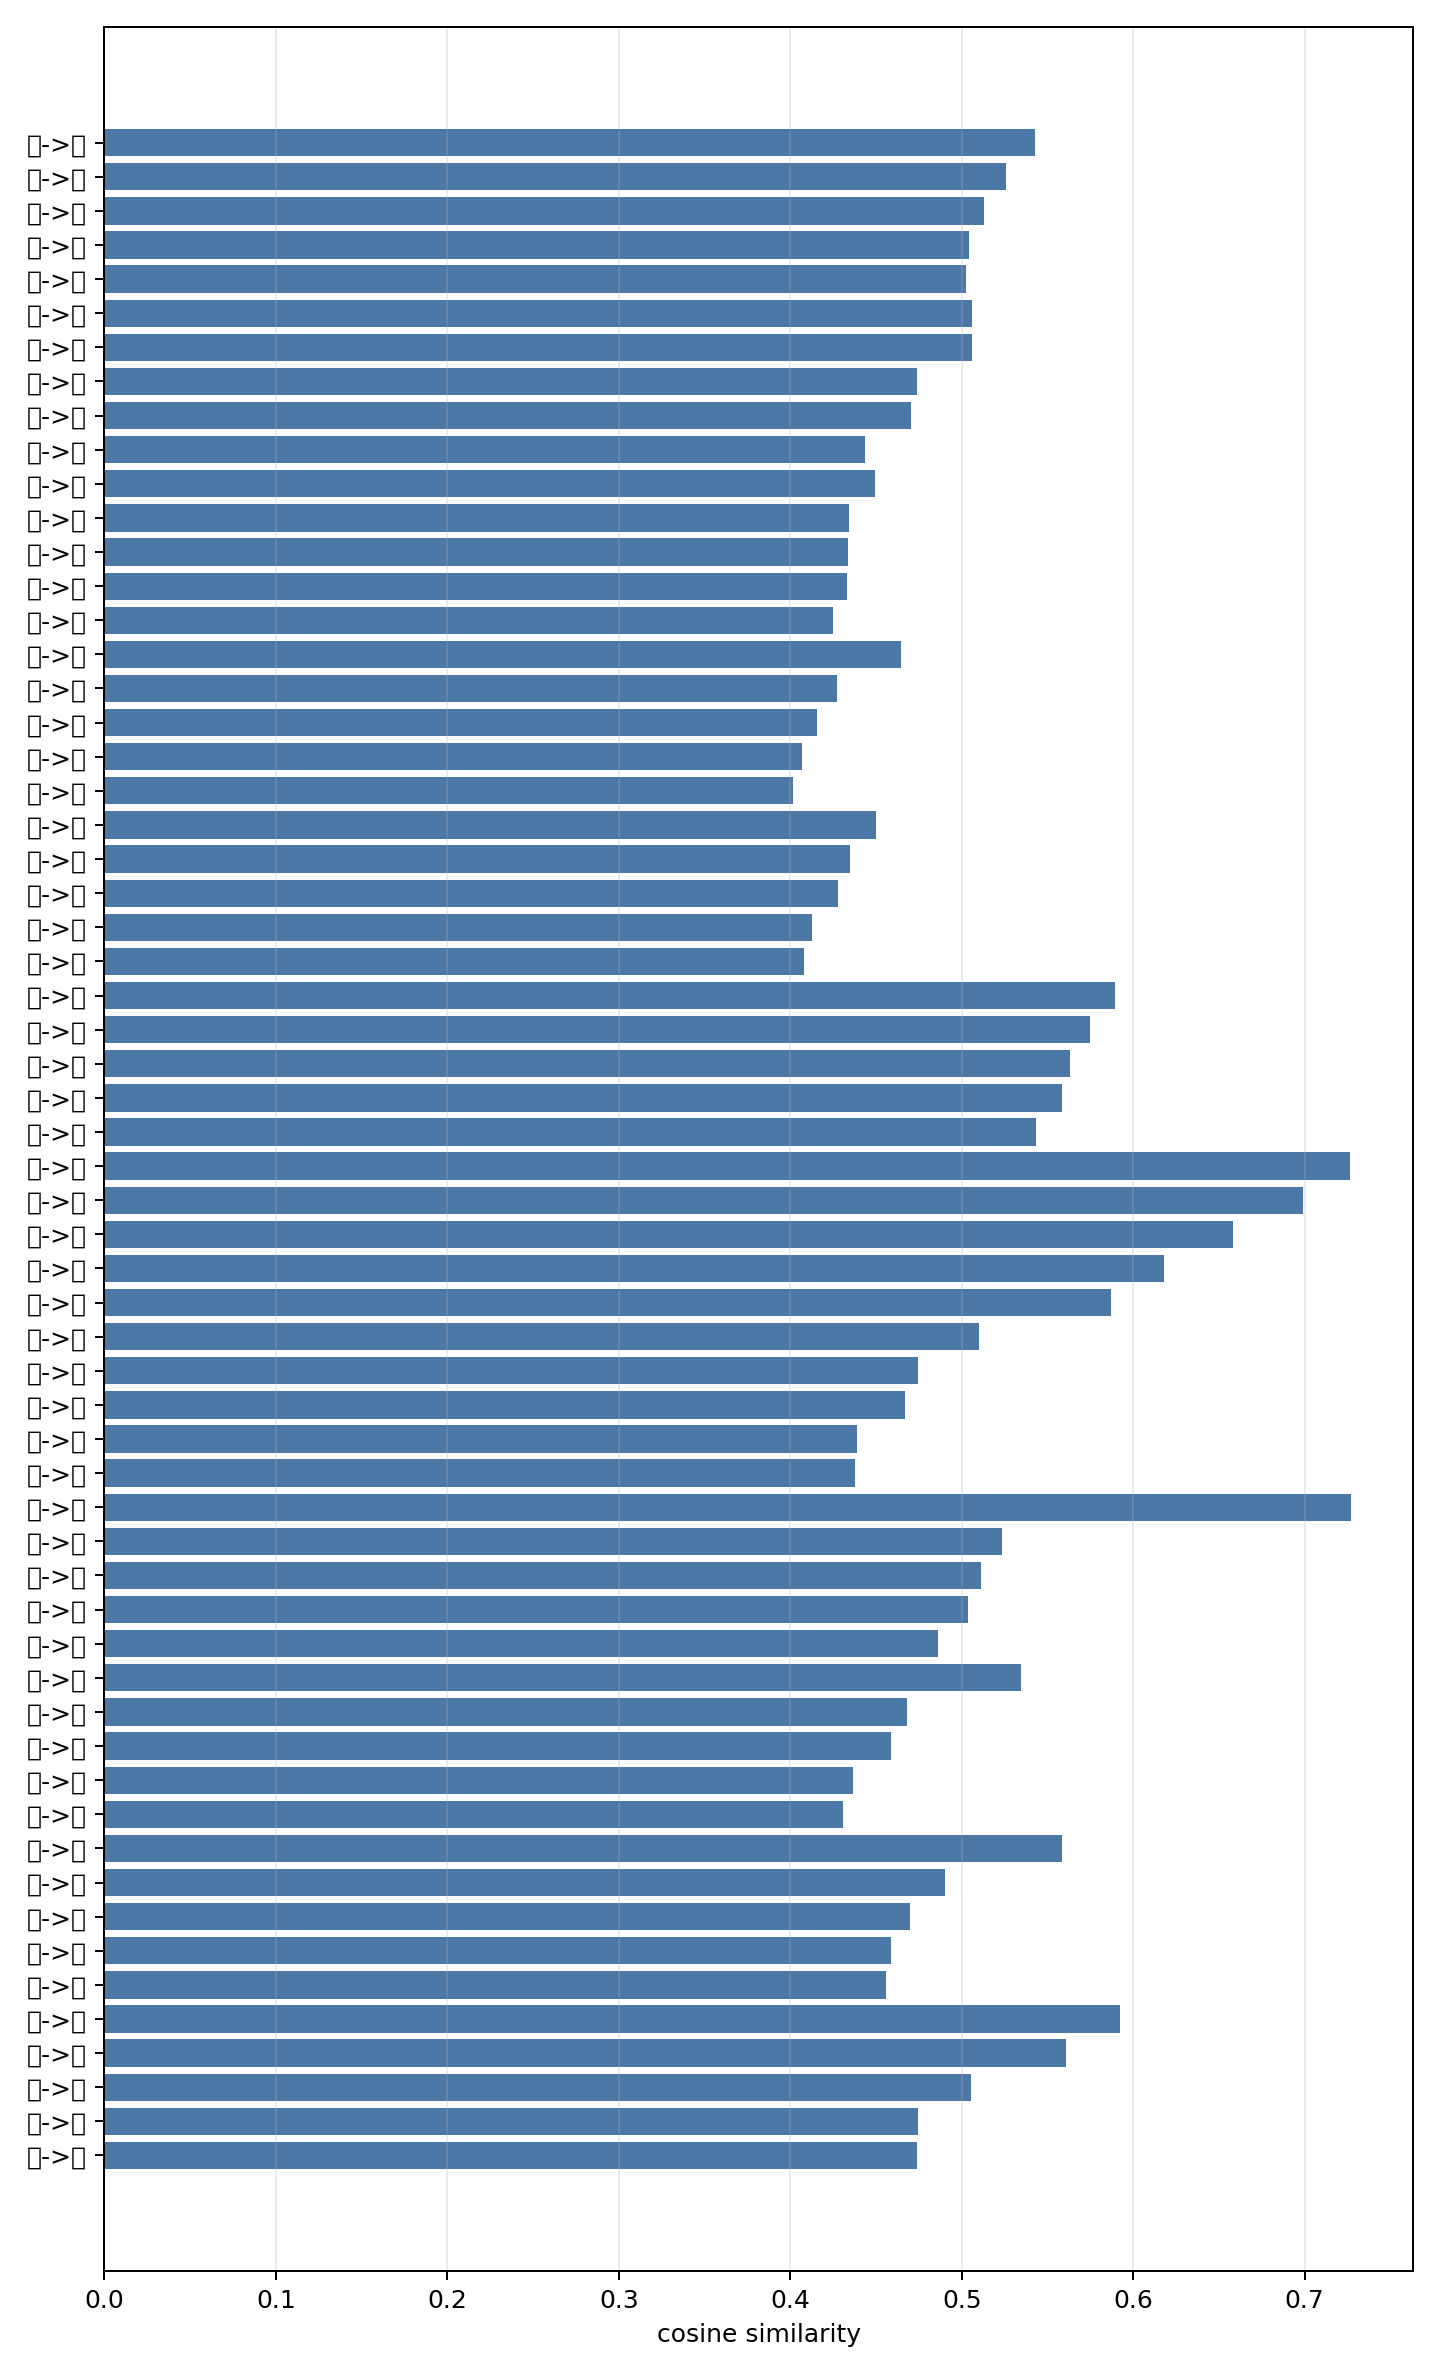
\includegraphics[width=\columnwidth]{results/word2vec/neighbors.png}}
{\fbox{\parbox{0.9\columnwidth}{\centering 服务器运行后生成 \texttt{results/word2vec/neighbors.png}}}}
\caption{Skip-gram 嵌入近邻相似度}
\end{figure}

\subsection{生成结果分析}
若模型学习有效，验证题目的生成答案应出现与真实答案相近的数字和单位。例如面积类问题常生成「畝」「步」「頃」等单位，分数约分类问题常生成「分之」结构，粟米换算题常生成粮食单位。即使小模型不能完全算对每一道题，只要在未见题目上稳定生成题型相关单位和数词，就说明它已经学习到《九章算术》中的局部知识模式。

\subsection{嵌入结果分析}
文本嵌入的近邻可以从另一个角度验证学习效果。理想情况下，「田」的近邻会包含「畝」「步」「廣」「從」等面积题相关字符；「分」的近邻会包含「之」「母」「子」等分数表达相关字符；「粟」「米」的近邻会围绕粮食换算术语。若近邻结果呈现这种聚类，说明 Skip-gram 模型捕捉到了古算文本中的上下文共现关系。

\section{不足与改进方向}
\begin{itemize}
  \item 本实验使用字符级模型，能处理古文编码和繁体字，但长距离推理能力有限；
  \item LSTM 主要学习文本模式，不能保证精确执行算术运算；
  \item 关键词命中率是弱指标，后续可人工构造更多保留题型但改变数字的测试题；
  \item 若服务器资源充足，可替换为 Transformer Decoder 或 Mamba，并增加上下文长度；
  \item 文本嵌入当前为字符级，可进一步加入基于规则的古汉语词表，训练词级 fastText。
\end{itemize}

\section{结论}
本实验完成了一个可复现的《九章算术》神经语言模型实验。字符级 LSTM 用于从题面续写「答曰」后的答案，Skip-gram 负采样模型用于学习数学文本嵌入。训练脚本会自动处理原始附件编码、抽取题答对、保存模型和结果图表。最终通过困惑度、答案关键词命中率、生成样例和嵌入近邻共同展示模型是否学习到《九章算术》中的知识。

\end{document}
